\newcommand{\btheta}{\boldsymbol{\theta}}
\newcommand{\data}{\boldsymbol{D}}
\newcommand{\documentname}{chapter}

\author[Brendon J. Brewer]{Brendon J. Brewer\\
Department of Statistics, The University of Auckland}

\chapter{Bayesian inference and computation: a beginner's guide}

\section{Introduction}
Most scientific observations are not sufficient to give us definite answers
to all of our questions. It is rare that we get a data set that {\it totally}
answers all of our questions with certainty. Even if that did happen, we would
quickly move on to other questions.
What a data set usually {\it can} do is make hypotheses more or less plausible,
even if we don't achieve total certainty.
Bayesian inference is a model of this
reasoning process, and also a tool we can use
to make quantitative statements about how much
uncertainty we should have about our conclusions. This takes the mystery out
of data analysis, because we no longer have to come up with a new method
every time we face a new problem. Instead, we simply specify exactly what
information we are going to use, and then compute the results.
In the last two decades, Bayesian inference has become immensely popular in
many fields of science, and astrophysics is no exception. Accessible textbooks
for those with a physics background are those by \citet{gregory} and
\citet{sivia}. For those with a statistical background, I recommend the book
by \citet{ohagan}.

Any particular application of Bayesian inference involves making choices
about what data you are analysing, what questions you are
trying to answer, and what assumptions you are willing to make.
Data analysis problems in astronomy vary widely, so in this \documentname~we
cannot cover a huge variety of examples. Instead, we will look at a small
number of examples. The assumptions we make in those examples will not always
be appropriate, but they should be sufficient to show you where the assumptions
enter and what you will need to consider when you work on a particular problem.

In principle, it's usually best to work with your data in the most
raw form possible, although this is often too difficult in practice.
Therefore, most scientists work with data that has been processed (by a ``pipeline'') and reduced to manageable size. To do Bayesian inference, you
need to specify what {\it prior information} you have (or are willing to
assume) about the problem, in addition to the data. Prior information is
necessary: what you can learn from a data set depends on what you know, for
example, about how it was produced.

Once you have your data, and have specified your prior information as well,
you are faced with the question of how to calculate the
results. Usually you want to calculate the {\it posterior distribution} for some
unknown quantities (also known as ``parameters'') given your data, which
describes your uncertainty about the , but takes into account the data.
Since we are often dealing with (potentially) complicated probability
distributions in high dimensional spaces, we need to {\it summarise} the
posterior distribution in an understandable way.
In certain problems, the summaries can be calculated analytically, but
numerical methods are more general, so will be the focus of this chapter.
The most popular and useful numerical techniques are the Markov Chain Monte
Carlo methods, often abbreviated as
MCMC\footnote{Some people claim that MCMC stands for
Monte Carlo Markov Chains, but they are wrong.}.
The rediscovery of MCMC in the 1990s
is one of the main reasons why Bayesian inference is so popular now.
While there were many strong philosophical arguments in favour of a Bayesian
approach before then, many people were still uncomfortable with the
subjective elements involved. However, once MCMC made it easy to compute the
consequences of Bayesian models more easily, people simply became more relaxed
about these subjective elements.

A huge variety of MCMC methods exists, and it would be
unwise to try to cover them all in this winter school. Therefore I will focus
on a small number of methods that are relatively simple to implement, yet quite powerful
and widely applicable. I will try to emphasise methods that are {\it general},
i.e. methods that will work okay on most problems you might encounter. One
disadvantage of this approach is that the methods we cover are not necessarily
the most efficient methods possible. If you're mostly interested in one
specific application, you'll probably be able to achieve better performance
by using a more sophisticated algorithm, or by taking advantage of the particular
properties of your problem.

There are many popular software packages (and many more unpopular ones)
available for doing Bayesian Inference, such as JAGS (Just Another Gibbs Sampler),
Stan, emcee, MultiNest, my own DNest3, and many more.
I won't be teaching you how to use any of these programs.
If you or your collaborators already use one of them, that's a great reason to
learn it! Please see the appendix for a discussion of the advantages and
disadvantages of these packages.

%JAGS is extremely convenient to use

\section{Python}
Due to its popularity and relatively shallow learning curve,
I will be using Python to implement the algorithms. The code I use will be
written so that it works in either Python 2 or 3. I will also assume that
each program has imported the following libraries:

\begin{minted}[mathescape,
               numbersep=5pt,
               gobble=2,
               frame=lines,
               framesep=2mm]{python}
  import numpy as np
  import numpy.random as rng
  import matplotlib.pyplot as plt
  import copy
\end{minted}



\section{Parameter Estimation}
Almost all data analysis problems can be interpreted as {\it parameter
estimation} problems. The term {\it parameter} has a few different meanings,
but you can usually just think of it as a synonym for {\it unknown quantity}.
When you learned how to solve equations in high school algebra,
you would have been able to find the value of an unknown quantity
(often called $x$) when you had
enough information to determine its value with certainty.
In science, we almost never have enough information to determine a quantity
without any uncertainty, which is why we need probability theory and Bayesian
inference.

We'll denote our unknown parameters by $\btheta$, which could be a single
parameter or perhaps a vector of parameters (e.g. the distance to a star
and the angular diameter of the star). To start, we
need to have some idea of the set of possible values we are considering. For
example, are the parameters integers? Real numbers? Positive real numbers?
In some examples, the definition of the parameters already restricts the set
of possible values. For example, {\it the proportion of extra-solar planets in
the Milky Way that contain life} cannot be less than 0 or greater than 1.
Strictly speaking, it has to be a rational number, but it probably won't make
much difference if we just say it's a real number between 0 and 1 (inclusive).
The distance to a star (measured in whatever units you like) is presumably a
positive real number, as is its angular diameter.
The set of possible values you're willing to consider is called the
{\it hypothesis space}.

To start using Bayesian inference, you need to assign a {\it probability
distribution} on the hypothesis space, which models your initial uncertainty
about the parameters. This probability distribution is called the {\it prior}.
We then use Bayes' rule, a consequence of the product rule of probability,
to calculate the {\it posterior} distribution, which describes our updated
state of knowledge about the values of the parameters, after taking the data
$D$ into account.

For a prior distribution $p(\btheta | I)$, and a sampling
distribution $p(\data | \btheta, I)$, Bayes' rule allows us to calculate
the {\it posterior distribution} for $\btheta$:
\begin{eqnarray}
p(\btheta | \data, I) &=& \frac{p(\btheta | I)p(\data | \btheta, I)}{p(\data | I)}.
\end{eqnarray}
The $I$ in this equation refers to background information and assumptions:
basically, it stands for everything you know about the problem apart from the
data. The result is a probability distribution for $\btheta$ which describes
our state of knowledge about $\btheta$ after taking into account the data.

The denominator, since it doesn't depend on $\btheta$, is a normalizing
constant. Since the posterior must integrate to one (or sum to one, if the
hypothesis space is discrete), we can write the denominator as:

\begin{eqnarray}
p(\data | I) &=& \int p(\btheta | I)p(\data | \btheta, I) \, d^N \btheta.
\end{eqnarray}


\begin{figure}
\begin{center}
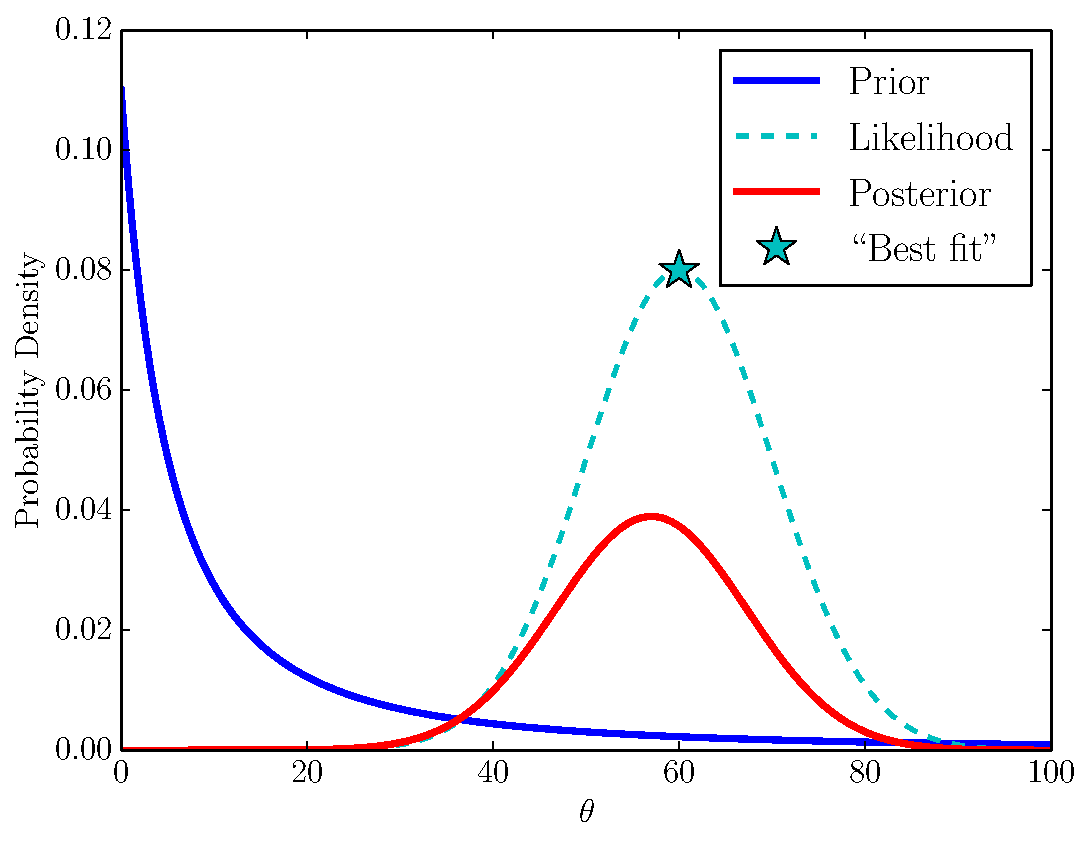
\includegraphics[scale=0.5]{bayes.pdf}
\caption{An example posterior distribution for a single parameter.
\label{fig:bayes}}
\end{center}
\end{figure}

\section{Transit Example}
To become more familiar with Bayesian calculations, we will work through a
simple curve-fitting example. Many astronomical data analysis problems can be
considered as examples of curve fitting. Consider a transiting exoplanet, like
one observed by {\it Kepler}. The light curve of the star will show an
approximately constant brightness as a function of time, with a small dip as
the exoplanet moves directly in front of the star. Clearly, real Kepler data
is much more complex than this example, as stars vary in brightness in
complicated ways, and the shape of the transit signal itself is more complex
than the model we'll use here. Nevertheless, this example contains all the
features and complications that will also arise in a more realistic analysis.

The data set, along with the true curve, is shown in 
Figure~\ref{fig:transit_data}. The equation for the true curve was:
\begin{eqnarray*}
\mu(t) &=& \left\{
\begin{array}{lr}
10, & 2.5 \leq t \leq 4.5\\
5,  & \textnormal{otherwise}.
\end{array}
\right.
\end{eqnarray*}

\begin{figure}
\begin{center}
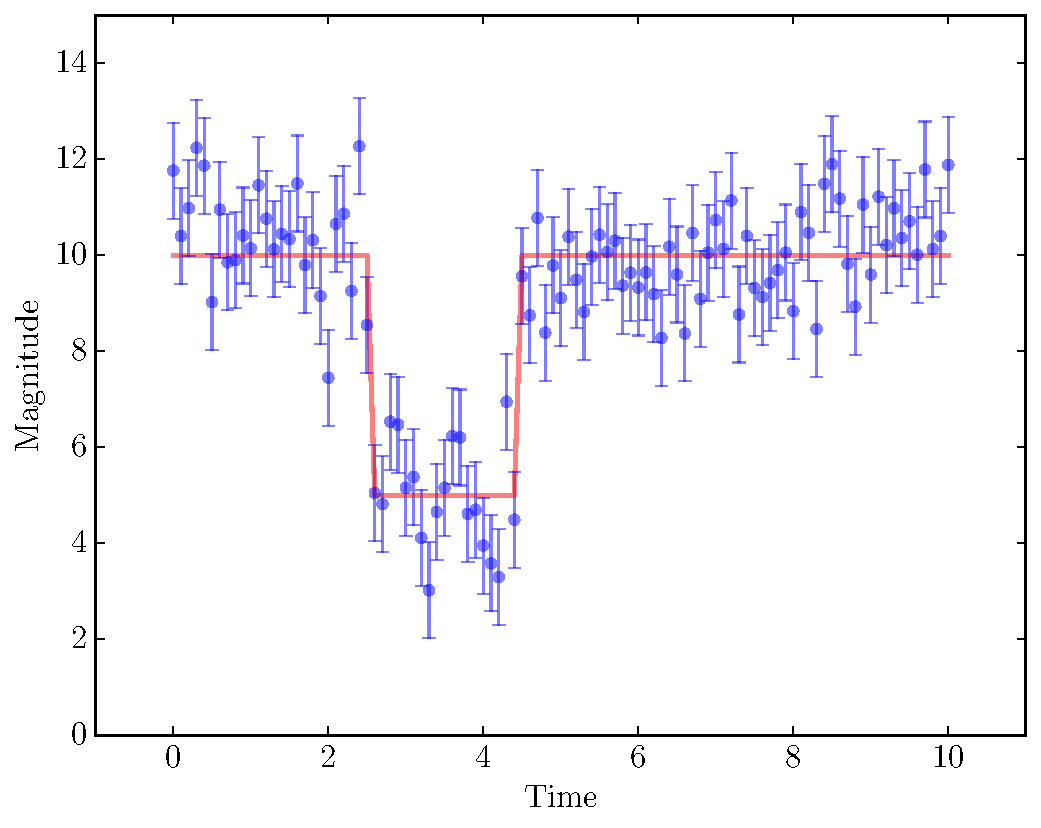
\includegraphics[scale=0.5]{../Code/transit_data.pdf}
\caption{The ``transit'' data set. The red curve shows the model prediction
based on the true values of the parameters.\label{fig:transit_data}}
\end{center}
\end{figure}

Let's assume that we didn't know this, but we did know the true curve
was a function of the following form:
\begin{eqnarray*}
\mu(t) &=& \left\{
\begin{array}{lr}
A, & (t_c - w/2) \leq t \leq (t_c + w/2)\\
A-b,  & \textnormal{otherwise}.
\end{array}
\right.
\end{eqnarray*}

We don't know the values of $A$, $b$, $t_c$, and $w$,
but we do know the data $D$. Applying Bayesian inference to this problem
involves calculating the posterior distribution for $A$, $b$, $t_c$, and $w$,
given the data $D$. For this specific setup, Bayes' rule states:

\begin{eqnarray}
p(A, b, t_c, w | D) &=& \frac{p(A, b, t_c, w)p(D | A, b, t_c, w)}{p(D)}
\end{eqnarray}

So, in order for the posterior distribution to be well defined, we need to
choose a prior distribution $p(A, b, t_c, w)$ for the parameters, and a
sampling distribution $p(D | A, b, t_c, w)$ for the data. Since the denominator
$p(D)$ is not a function of the parameters, it plays the role of a normalising
constant that ensures the posterior distribution integrates to 1, as any
probability distribution must.

\subsection{Sampling Distribution}
The {\it sampling distribution} is the probability distribution would assign
for the data, if we knew the true values of the parameters.
In many situations, it is conventional to assign a normal distribution
(also known as a gaussian distribution) to each data point, where the mean
of the normal distribution is the noise-free model prediction, and the
standard deviation of the normal distribution is given by the size of the
error bar. Later, we will see how to relax these assumptions in a useful way.
The probability density for the data given the parameters (i.e. the sampling
distribution) is:

\begin{eqnarray}
p(D | A, b, t_c, w) &=& \prod_{i=1}^N \frac{1}{\sigma_i \sqrt{2\pi}}
\exp\left[-\frac{1}{2\sigma_i^2}\left(D_i - \mu(t_i)\right)^2\right]\label{eq:gaussian}
\end{eqnarray}
This is a product of $N$ terms, one for each data point. We have assumed that
each data point is {\it independent} (given the parameters). That is, if we
knew the parameters and some of the data points, in predicting other data points
we would be able to make use of the parameters, but not the data points we
already knew. When the data is known, Equation~\ref{eq:gaussian} becomes a
function of the parameters called the likelihood function. The curve predicted
by the model, here written as $\mu(t_i)$ (where I have suppressed the implicit
dependence on the parameters, for brevity), provides the mean of the gaussian
distribution. It is important to remember that the independence assumption we
used here is not an assumption about the actual data set, but an assumption
about our prior information about the data set.

Equation~\ref{eq:gaussian} is the sampling distribution
(and the likelihood function) for our problem, but it
was fairly cumbersome to write down. Statisticians have developed a shorthand
notation for writing down probability distributions, which is extremely useful
for communicating what assumptions you are making, without having to write down
the entire equation for the probability density. To communicate
Equation~\ref{eq:gaussian}, we can simply write

\begin{eqnarray}
D_i \sim \mathcal{N}\left(\mu(t_i), \sigma_i^2\right)
\end{eqnarray}
i.e. each data point has a normal distribution with mean $\mu(t_i)$ (which
depends on the parameters) and standard deviation $\sigma$. For the normal
distribution, it is traditional to write the {\it variance} (standard deviation
squared) as the second argument.

\subsection{Priors}
Now we need a prior for the unknown parameters $A, b, t_c$, and $w$. This is
a prior over a four dimensional parameter space. To simplify things, we can
assign independent priors for each parameter, and multiply these together
to produce the joint prior:
\begin{eqnarray}
p(A, b, t_c, w) &=& p(A)p(b)p(t_c)p(w).
\end{eqnarray}
This prior distribution models our uncertainty about the parameters before
taking into account the data. The independence assumption implies that if we
were to learn the value of one of the parameters, this wouldn't tell us anything
about the others. This may or may not be realistic in a given application, but
it is a useful starting point.

Another useful starting point for priors is the uniform distribution.
\begin{eqnarray}
A &\sim& U(-100, 100)\\
b &\sim& U(0, 10)\\
t_c &\sim& U(t_{\rm min}, t_{\rm max})\\
w &\sim& U(0, t_{\rm max} - t_{\rm min})
\end{eqnarray}
The full expression for the probability density is:
\begin{eqnarray}
p(A, b, t_c, w) &=&
\left\{
\begin{array}{lr}
\frac{1}{2000\left(t_{\rm max} - t_{\rm min}\right)^2}, & (A, b, t_c, w) \in S\\
0, & \textnormal{otherwise}
\end{array}
\right.
\end{eqnarray}
where $S$ is the set of allowed values. Even more simply, we can ignore the
normalising constant and the prior boundaries and just write
\begin{eqnarray}
p(A, b, t_c, w) &\propto& 1.
\end{eqnarray}




\section{Markov Chain Monte Carlo}
{\it Monte Carlo} methods allow us to calculate any property of a probability
distribution that is an expectation value. For example, if we have a
single variable
$x$ with a probability density $p(x)$, the expected value is
\begin{eqnarray}
\mathds{E}(x) &=& \int_{-\infty}^{\infty} x p(x) \, dx 
\end{eqnarray}
which is a measure of the ``center of mass'' of the probability distribution.

If we had a set of points $\{x_1, x_2, ..., x_N\}$ ``sampled from'' $f(x)$,
we could replace the integral with a simple average:
\begin{eqnarray}
\mathds{E}(x) &\approx& \frac{1}{N} \sum_{i=1}^N x_i.
\end{eqnarray}
In one dimension, this may not seem very useful. Evaluating a one dimensional
integral analytically is often possible, and doing it numerically using the
trapezoidal rule (or a similar approximation) is quite straightforward.
However, Monte Carlo really becomes useful in higher dimensional problems.
For example, consider a problem with five unknown quantities with probability
distribution $p(a, b, c, d, e)$, and suppose we want to know the probability
that $a$ is greater than $b + c$. We could do the integral
\begin{eqnarray}
P(a > b + c) &=& \int p(a, b, c, d, e) \mathds{1}\left(a > b + c\right) \, da \, db \, dc \,dd \,de 
\end{eqnarray}
where $\mathds{1}\left(a > b + c\right)$ is a function that is equal to one
where the condition is satisfied and zero where it isn't. However, if we could
obtain a sample of points in the five dimensional space, the Monte Carlo
estimate of the probability is simply
\begin{eqnarray}
P(a > b + c) &\approx& \frac{1}{N}\sum_{i=1}^N \mathds{1}\left(a_i > b_i + c_i\right)
\end{eqnarray}
which is just the fraction of the samples that satisfy the condition.

Another important use of Monte Carlo is marginalisation. Suppose again we had
a probability distribution for five variables, but we only cared about one of
them. For example, the marginal distribution of $a$ is given by
\begin{eqnarray}
p(a) &=& \int p(a, b, c, d, e) \, db \, dc \, dd \, de
\end{eqnarray}
which describes your uncertainty about $a$, rather than your uncertainty about
all of the variables. This integral might be analytically intractable. With
Monte Carlo, if you have samples in the five dimensional space but you only
look at the first coordinate, then you have samples from $p(a)$. This is
demonstrated graphically in Figure~\ref{fig:marginalisation}.

\begin{figure}
\begin{center}
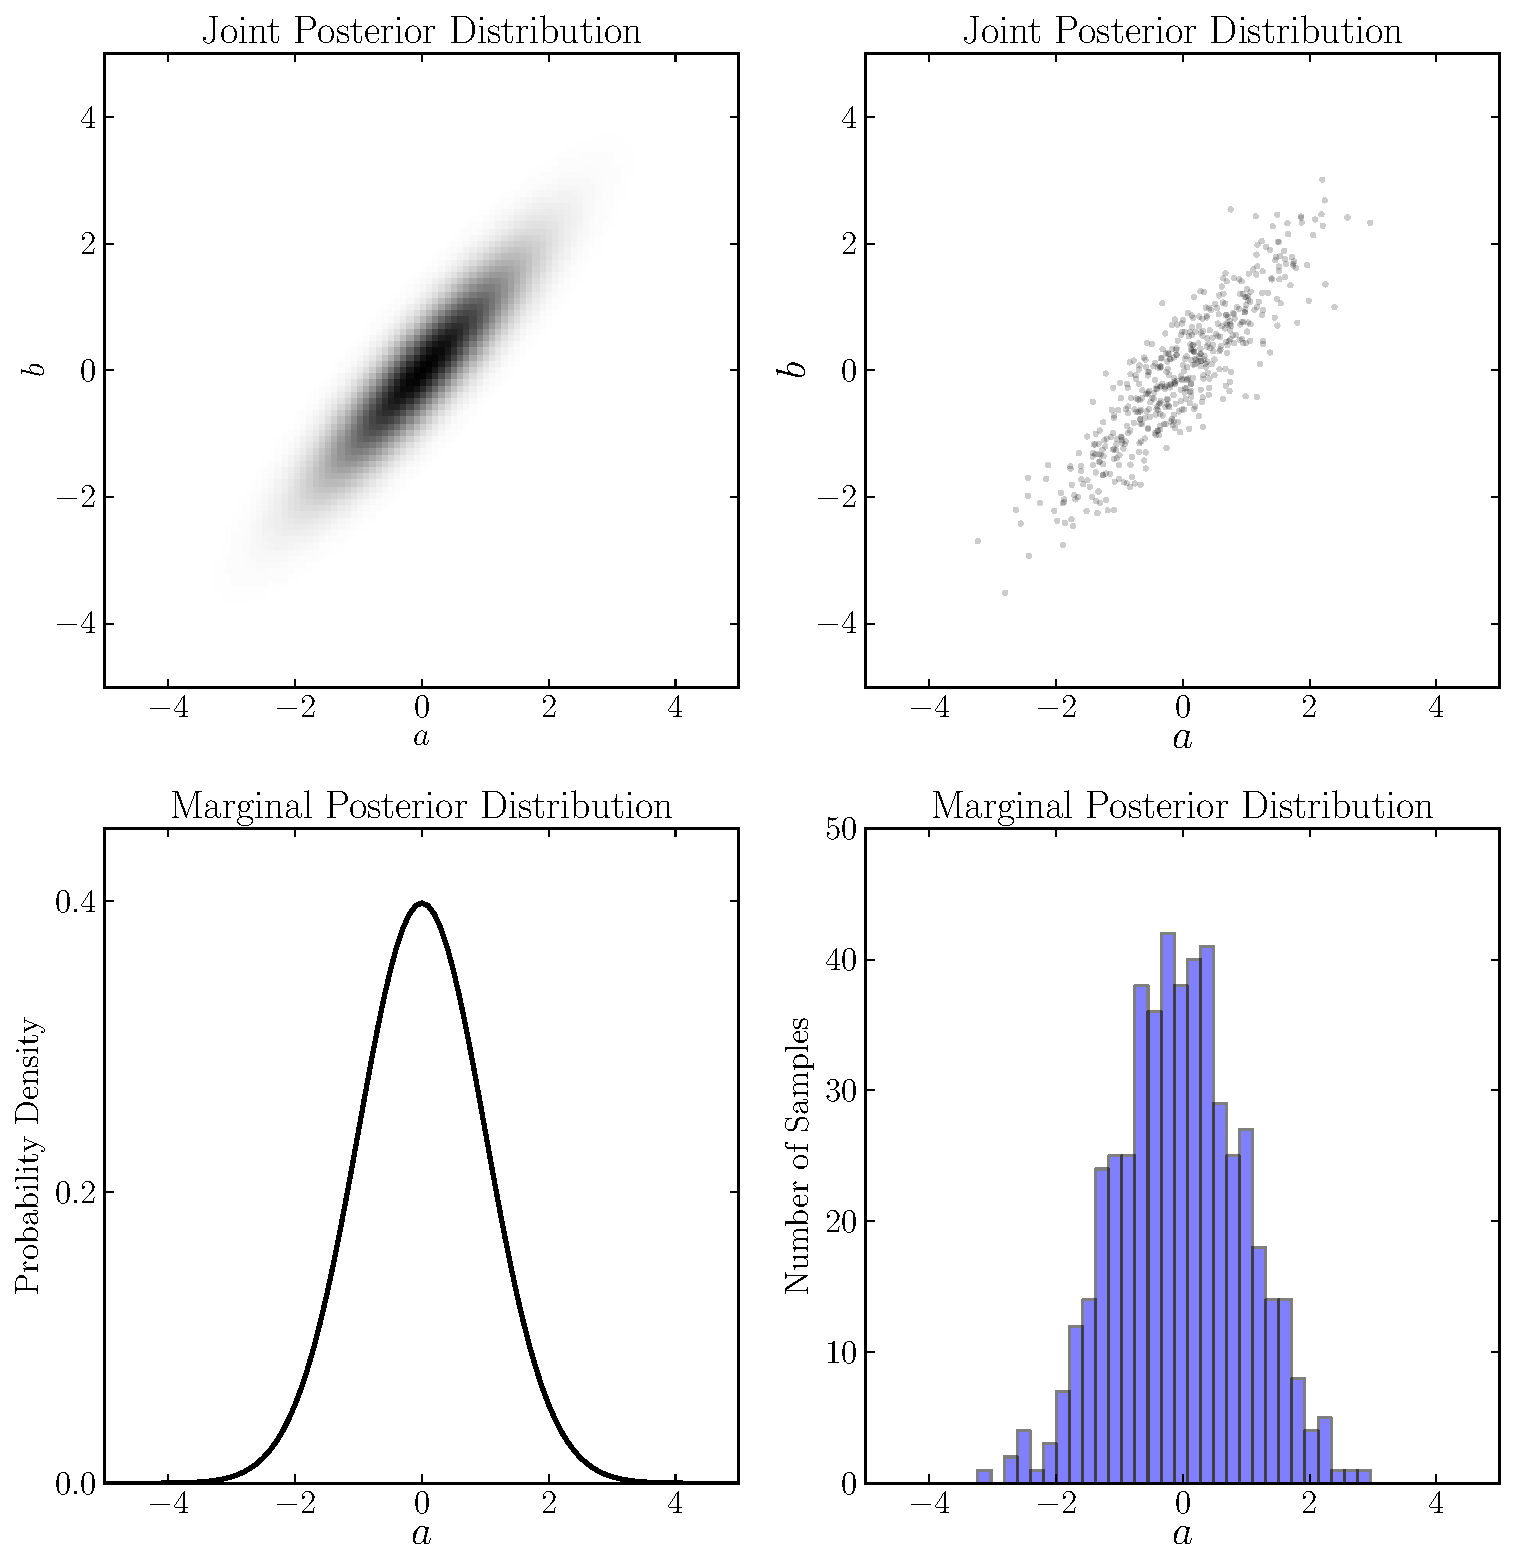
\includegraphics[scale=0.5]{../marginalisation.pdf}
\caption{An example posterior distribution for two parameters $a$ and $b$.
Figure taken from ...
\label{fig:marginalisation}}
\end{center}
\end{figure}

In Bayesian inference, the most important probability distribution is the
posterior distribution for the parameters. We would like to be able to
generate samples from the posterior, so we can compute probabilities,
expectations, and other summaries easily. Markov Chain Monte Carlo allows us
to generate these samples.

\subsection{The Metropolis Algorithm}
The Metropolis-Hastings algorithm, also known as the Metropolis algorithm, is
the oldest and most fundamental MCMC algorithm.
It is quite straightforward to implement, and works well on many problems.
The version of the Metropolis algorithm presented here is sometimes called
{\it random walk} Metropolis. More sophisticated choices are possible,
but usually require problem-specific knowledge.

Consider a problem with a single unknown
parameter $x$. If the prior is some density $\pi(x)$ and the likelihood
function is $\mathcal{L}(x)$, then the posterior distribution will be
proportional to $\pi(x)\mathcal{L}(x)$. The normalising constant
$Z = \int \pi(x) \mathcal{L}(x) \, dx$ is unknown,
but the Metropolis algorithm doesn't need to know it: all we need is the
ability to evaluate $\pi$ and $\mathcal{L}$ at a given position in the parameter space.

The Metropolis algorithm can be summarised as follows:
\begin{itemize}
\item Choose a starting position $x$, somewhere in the parameter space.
\item Generate a proposed position $x'$ from a proposal distribution
$q(x'|x)$.
\item With probability
$\alpha=\min\left(1, \frac{q(x|x')}{q(x'|x)}\frac{\pi(x')}{\pi(x)}\frac{\mathcal{L}(x')}{\mathcal{L}(x)}\right)$, accept the proposal
(i.e. replace $x$ with $x'$). Otherwise, do nothing.
\end{itemize}

The ``random walk'' proposal generates a proposed value $x'$ from a normal
(gaussian) distribution centered around the current position $x$. The user
is free to choose the width of the normal distribution. Here is a Python code
snippet showing a proposal with width {\tt L}:

\begin{minted}[mathescape,
               numbersep=5pt,
               gobble=2,
               frame=lines,
               framesep=2mm]{python}
  # Generate a proposal
  proposal = x + L*rng.randn()
\end{minted}

The performance of the Metropolis algorithm depends quite strongly on
the width of the proposal distribution. If the width is too small, most moves
will be accepted, but won't move very far. If the width is too large, most
moves will be rejected, so you'll end up stuck in one place. Some authors
recommend using preliminary runs to find an optimal width. Instead, I recommend
that you use a mixture of widths. Basically, every time we make a proposal,
the width is drawn from some range, rather than being constant. The biggest
possible width we would ever want should be roughly the order of magnitude of
the width of the prior (since the posterior is usually narrower than the
prior).
\begin{minted}[mathescape,
               numbersep=5pt,
               gobble=2,
               frame=lines,
               framesep=2mm]{python}
  # A heavy-tailed proposal distribution
  # Generate a standard deviation
  L = 10.**(1.5 - 6.*rng.rand())

  # Use the standard deviation for the proposal
  proposal = x + L*rng.randn()
\end{minted}
With this proposal, the minimum width is
$10^{-4.5} \approx 3.16 \times 10^{-5}$, and the maximum width is
$10^{1.5} \approx 31.6$. The effective proposal distribution is now very heavy-tailed. As long as a good width is somewhere within our range, things should be
okay.

When there are multiple parameters (almost always, since MCMC isn't necessary
on single parameter problems!), we need to decide how to construct the proposal.
There are two main ways to do this. The first is that the proposal is to
change all of the parameters simultaneously. This tends to be inefficient in
high dimensions, because the only proposals that are likely to be accepted
are those that change the parameter values only slightly: in a high dimensional
space, there are many bad directions to travel, and not very many good ones.
Usually, it's better to propose to change a subset of the parameters, or even
just a single parameter. In Python, a function that takes a numpy vector of
parameters and input and returns a proposed value for the parameters is
specified below.

\begin{minted}[mathescape,
               numbersep=5pt,
               gobble=2,
               frame=lines,
               framesep=2mm]{python}
def proposal(params):
  """
  Generate new values for the parameters, for the Metropolis algorithm.
  """
  # Copy the parameters
  new = copy.deepcopy(params)

  # Which one should we change?
  which = rng.randint(num_params)
  new[which] += jump_sizes[which]*10.**(1.5 - 6.*rng.rand())*rng.randn()
  return new
\end{minted}
This function relies on {\tt num\_params} being the number of parameters,
and a vector {\tt jump\_sizes}, of length {\tt num\_params}, which specifies
the prior width for each parameter.


\subsection{Useful Plots}
After running the Metropolis algorithm (or any other MCMC method), there are
several useful plots that you should make.

\begin{figure}
\begin{center}
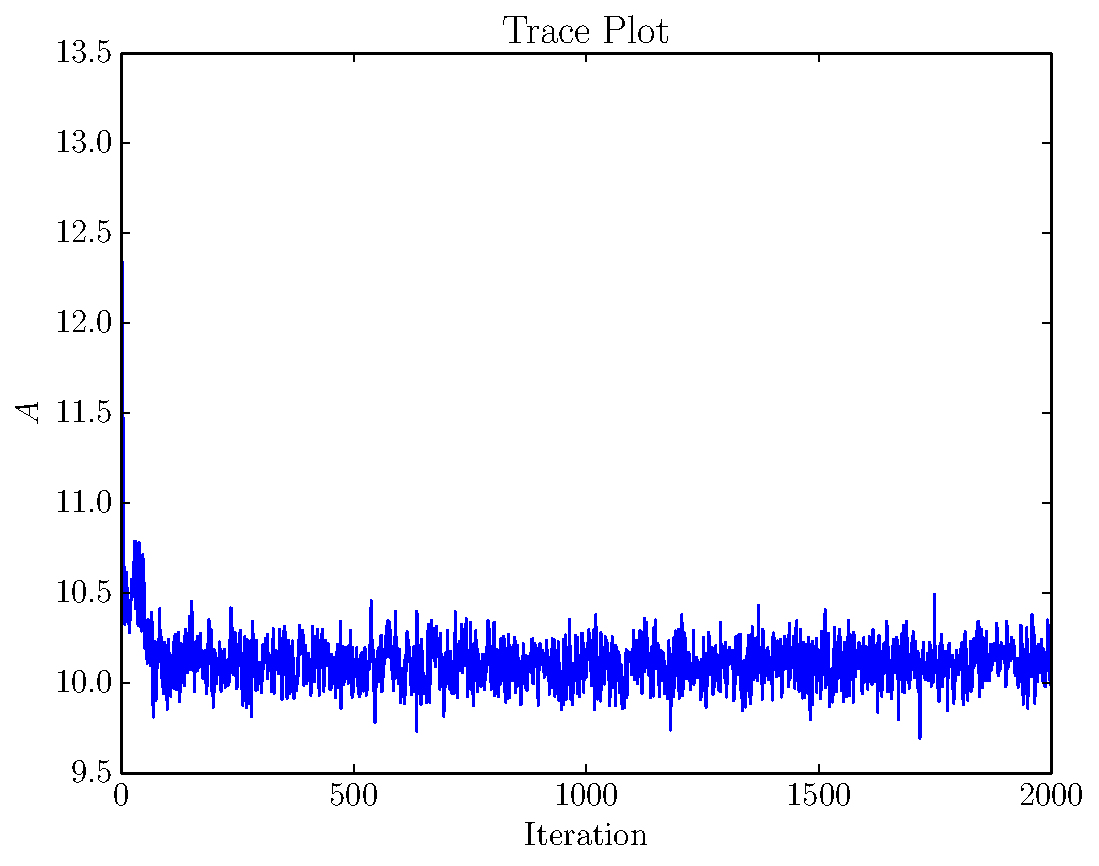
\includegraphics[scale=0.5]{trace_plot.pdf}
\caption{A ``trace plot''. At the beginning, because of the initial conditions
of the algorithm, the results start in a region of parameter space that has
very low probability. This initial phase is often called the ``burn-in'', and
should be excluded from any subsequent calculations.\label{fig:trace_plot}}
\end{center}
\end{figure}

\begin{figure}
\begin{center}
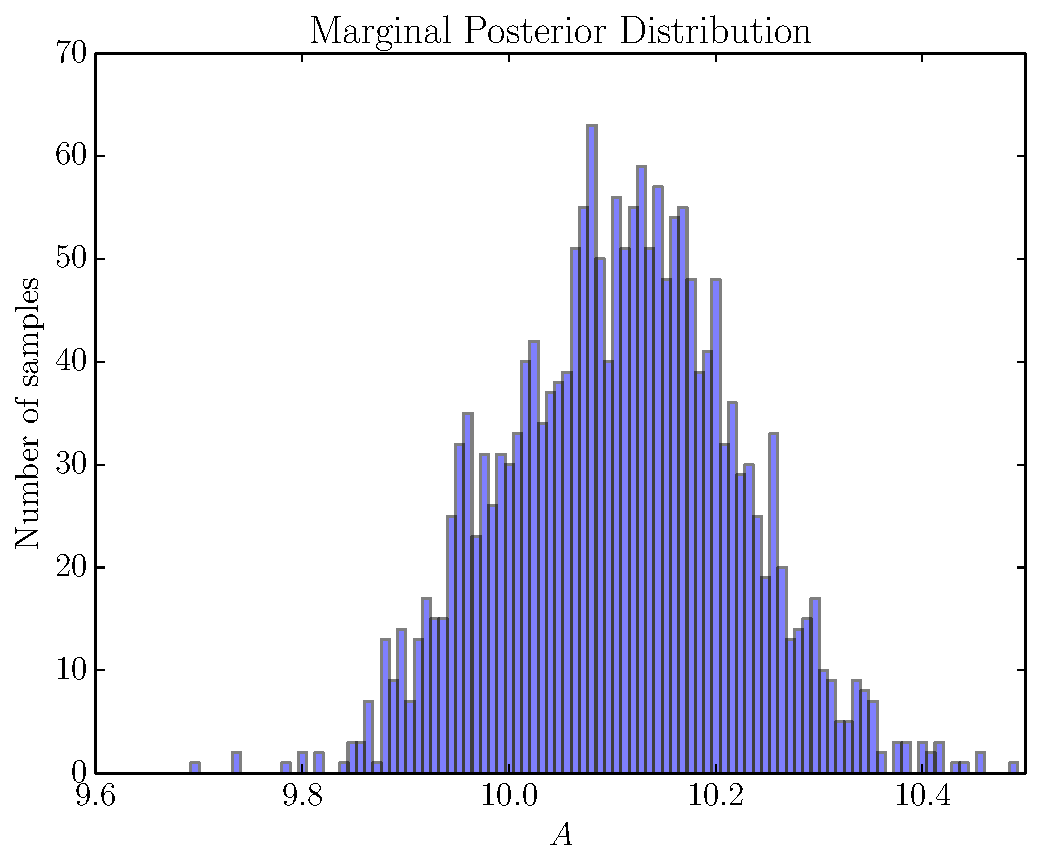
\includegraphics[scale=0.5]{marginal_posterior.pdf}
\caption{\label{fig:marginal_posterior}}
\end{center}
\end{figure}

\begin{figure}
\begin{center}
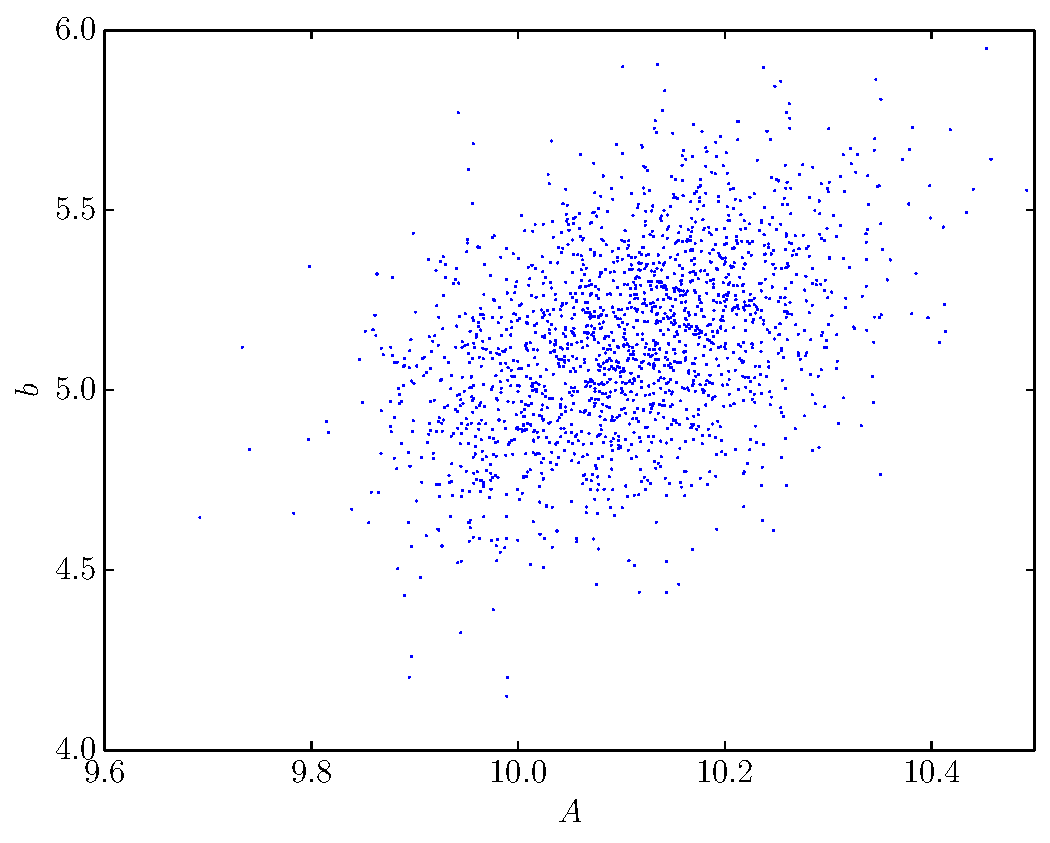
\includegraphics[scale=0.5]{joint_posterior.pdf}
\caption{\label{fig:joint_posterior}}
\end{center}
\end{figure}


\subsection{Posterior Summaries}
A probability distribution, such as the posterior,
can potentially be arbitrarily complicated. For communication purposes, it is
usually easier to summarise the distribution by a few numbers. The most common
summaries are point estimates (i.e. a single estimate for the value of the
parameter, such as ``we estimate $\theta$ = 0.43'') and intervals (e.g.
the probability that $\theta \in [0.3, 0.5]$ is 68\%).

Thankfully, most of these summaries are trivial to calculate from Monte Carlo
samples, such as those obtained from MCMC. The most popular point estimate is
the posterior mean, which is approximated by the arithmetic mean of the samples.
The posterior median can also be easily approximated by the arithmetic median
of the samples.

\begin{minted}[mathescape,
               numbersep=5pt,
               gobble=2,
               frame=lines,
               framesep=2mm]{python}
  post_mean = np.mean(samples)
  post_median = np.median(samples)
\end{minted}

There are some theoretical arguments, based on decision theory, that provide
guidance about which point estimate is better under which circumstances.

To compute a credible interval (the Bayesian version of a confidence interval),
you find quantiles of the distribution. For example, if we want to find an
interval that contains 95\% of the posterior probability, the lower end of the
interval is the parameter value for which 2.5\% of the samples are lower.
Similarly, the upper end of the interval is the value for which 2.5\% of the
samples are higher (i.e. 97.5\% are lower). The simplest way to implement this
calculation is by sorting the samples, as shown below.

\begin{minted}[mathescape,
               numbersep=5pt,
               gobble=2,
               frame=lines,
               framesep=2mm]{python}
  sorted_samples = np.sort(samples)
  # Left and right end of interval
  left = sorted[int(0.025*len(sorted))]
  right = sorted[int(0.975*len(sorted))]
\end{minted}

This kind of interval is sometimes called a {\it centered} credible interval,
because the same amount of probability lies outside the interval on each side.
In astronomy, it is more common to quote a 68\% credible interval, which is
equivalent to ``plus or minus one posterior standard deviation'' if the
posterior is gaussian.

\section{Assigning Prior Distributions}
There are only really two open problems in
Bayesian inference. The first is how to assign sensible prior distributions
(and sampling distributions) in different circumstances, and the
second is how to calculate the results efficiently. With regard to the first
problem ,it is sometimes said that there are two different kinds of Bayesian inference,
{\it subjective} and {\it objective}, with different methods for choosing
priors. My view is that Bayesian describes a {\it hypothetical}
state of prior knowledge, held by an idealised reasoner. When we apply
Bayesian inference, we are studying how the idealised reasoner would update
their state of knowledge based on the information we explicitly put into the
calculation.

In many cases, we can just use simple ``default'' choices for the prior and
the sampling distribution (e.g. a uniform prior for a parameter, and a
``gaussian noise'' assumption for the data). A lot of analyses work just fine
with these assumptions, and taking more care wouldn't change the results in
any important way. However, occasionally it makes sense to spend a lot of
time and effort thinking about the prior distributions.
So-called subjective Bayesians, who are not
necessarily experts in the fields of their clients, conduct elaborate interviews
with experts to try and create a prior that models the experts' beliefs well.
This process is called {\it elicitation}.
For example, consider the Intergovernmental Panel on Climate Change (IPCC),
who periodically write immense reports summarising humanity's state of knowledge
about global warming.
Consider the question ``{\it How much will the global average temperature
increase in the next 100 years?}''. This is exactly the kind of situation where
elicitation of an expert's probabilities is very important: a lot is known,
and a lot is at stake. In this situation, it wouldn't be very wise to rely on
convenient ``vague'' priors!

On the other hand, so-called ``objective'' Bayesians search for principles
based on symmetry or other arguments, which can help choose a prior that is
an appropriate choice to describe a large amount of ignorance. Some examples
include the principle of indifference, the Jeffreys prior, reference priors,
default priors, and transformation groups.

\subsection{Probability distributions have consequences}
When you assign prior distributions, it is more easy than you might expect to
build in an assumption that you don't really agree with. This is especially
true in high dimensional problems. Imagine that you wanted to infer the mass
$M$ of a galaxy. A suitable ``ignorance'' prior might be the uniform distribution
between $10^{5}$ and $10^{15}$ solar masses:
\begin{eqnarray}
M \sim U(10^{5}, 10^{15})
\end{eqnarray}
However, this has an unfortunate feature: it implies that the prior probability
of $M$ being greater than $10^{14}$ is 0.9, and the probability of $M$ being
greater than $10^{12}$ is 0.999, which seems overly confident, when we were
trying to describe ignorance! In astronomy,
we are often in the situation of having to ``put our error bars in the
exponent''. A prior that has this property is the ``log-uniform'' distribution
(named by analogy with the lognormal distribution, and sometimes incorrectly
called a Jeffreys prior), which assigns a uniform distribution to the logarithm
of the parameter. If we replace the uniform prior by
\begin{eqnarray}
\log(M) \sim U(\log(10^{5}), \log(10^{15}))
\end{eqnarray}
then the prior probabilities are more moderate: $P(M > 10^{14}) = 0.1$,
$P(M > 10^{12}) = 0.3$, and so on.



\section{What is the data?}
It can sometimes be helpful to think carefully about exactly what your data set
contains, and whether it is all ``data'' in the sense of Bayesian inference.
In the transit example, we chose a sampling distribution for the data, but this
sampling distribution was for the $y$-values of the data
(the flux measurements). Note that we never assigned a probability distribution
for the {\it times} of the data points, even though we might think of that as
part of the data (it's probably in the same file as the measurements, after all).
In fact, because we didn't assign a probability distribution for it, the
timestamps were not data at all, but part of the prior information $I$.
Therefore, it is completely justifiable to use the timestamps when assigning
the prior and the sampling distribution.




\section{Birth and death moves}
Sometimes, when you are trying to fit a model to data, there is uncertainty
not just about the values of the model parameters, but also how many model
parameter exist in the first place. One example is
the radial velocity technique for detecting extra-solar planets
\citep{gregory}, where the goal is to fit a signal to a sparse data set, where
we don't know how many components (planets) there are.



\section{Model Selection and Nested Sampling}
Nested Sampling is a Monte Carlo algorithm introduced by \citet{skilling}.
Several variants of Nested Sampling exist, and most of them are somewhat
complicated. Here, I will present a simple version of Nested Sampling which
is sufficient to solve a wide range of problems. This approach is similar to
the one presented in the introductory textbook by \citet{sivia}.

Many more complex and sophisticated versions of
Nested Sampling exist, such as the popular MultiNest \citep{multinest},
my own Diffusive Nested Sampling \citep{dnest}, and several others. These
algorithms, while all based on the insights of \citet{skilling}, are very
different in detail. See the appendix for more details.

Consider two different models $M_1$ and $M_2$ which are mutually exclusive
(they can't both be true).
Suppose $M_1$ has parameters
$\btheta_1$, and $M_2$ has its own parameters $\btheta_2$. The methods
described previously can be used to calculate the posterior distribution for
$M_1$'s parameters:
\begin{eqnarray}
p(\btheta_1 | D, M_1) &=& \frac{p(\btheta_1 | M_1)p(D | \btheta_1, M_1)}
{p(D | M_1)}
\end{eqnarray}
You can also fit model $M_2$ to the data, i.e. get the posterior distribution
for $M_2$'s parameters:
\begin{eqnarray}
p(\btheta_2 | D, M_2) &=& \frac{p(\btheta_1 | M_2)p(D | \btheta_2, M_2)}
{p(D | M_2)}
\end{eqnarray}
This is all very well, but you might want to know whether $M_1$ or $M_2$ is
more plausible overall, given your data. That is, you want the posterior
probabilities $P(M_1 | D)$ and $P(M_2 | D)$.

In this situation, it's usually easier to calculate the ratio of the two
posterior probabilities, which is sometimes called the {\it posterior odds
ratio}:
\begin{eqnarray}
\frac{P(M_2 | D)}{P(M_1 | D)} &=& \frac{P(M_2)}{P(M_1)}
\times \frac{P(D | M_2)}{P(D | M_1)}
\end{eqnarray}

As you might expect, the posterior odds for $M_2$ over $M_1$ depends on the
prior odds: was $M_2$ more plausible than $M_1$ before taking into account the
data? The other ratio is a ratio of likelihoods, how probable was the data
assuming $M_2$ vs assuming $M_1$? These likelihoods aren't the likelihoods
for a specific value of the parameters, but instead likelihoods for the model
as a whole. To distinguish this kind of likelihood from the standard kind (which
is a function of the model parameters), the term {\it marginal likelihood} or
{\it evidence} is used. The marginal likelihood for $M_1$ is:
\begin{eqnarray}
p(D | M_1) &=& \int p(\btheta_1 | M_1) p(D | \btheta_1, M_1) \, d^{N_1} \btheta_1
\label{eq:marginal_likelihood}
\end{eqnarray}
To do model selection, we need this as well as the marginal likelihood for
$M_2$:
\begin{eqnarray}
p(D | M_2) &=& \int p(\btheta_2 | M_2) p(D | \btheta_2, M_2) \, d^{N_2} \btheta_2
\end{eqnarray}
Marginal likelihoods are integrals over the parameter space. They are
expected values, but they are not expected values with respect to the posterior
distribution, but rather the prior. Therefore, we cannot use standard MCMC
methods (at least in any simple way) to calculate the marginal likelihood.

A Monte Carlo approach that samples from the prior distribution will also fail
in most cases. The likelihood function $p(D | \btheta_1, M_1)$ in
Equation~\ref{eq:marginal_likelihood} is usually sharply peaked in a very
small region of parameter space. The integral will be dominated by the high values
of the likelihood in the tiny region, yet a Monte Carlo approach based on
sampling the prior will almost certainly not give any samples in the important
region.

\section{Appendix: Notation for Probability Distributions}
There are two main types of notation that are used in probability theory. The
first type is mathematically correct and conceptually
clear, yet results in equations that are very large, complicated,
and difficult to read.
The second type is a very compact notation which makes equations a lot
shorter and easier to read, but could be misinterpreted if you are not used to
it. I prefer the compact notation, but to prevent any misunderstandings
I'll describe both below.

Suppose we're about to flip a coin $N$ times, and are interested in the
quantity $X$, the number of times the result is heads. According
to the standard assumptions, the possible values for $X$ are the integers from 0
to 10, and the probability distribution for $X$ is given by
a binomial distribution:

\begin{eqnarray}
P(X = x) &=& \left(\begin{array}{cc}10\\ x\end{array}\right)
\left(\frac{1}{2}\right)^x\left(\frac{1}{2}\right)^{10 - x}\\
&=& \left(\begin{array}{cc}10\\ x\end{array}\right)
\left(\frac{1}{2}\right)^{10}
\end{eqnarray}
The equation gives us all the probabilities we want, i.e. $P(X=0)$, $P(X=1)$,
and so on. The lower case $x$ is a dummy variable: like the index in a sum, it
can be replaced by any other symbol and the equation still holds. For example,
replacing $x$ with $a$ gives:
\begin{eqnarray}
P(X = a) &=& \left(\begin{array}{cc}10\\ a\end{array}\right)
\left(\frac{1}{2}\right)^{10}.
\end{eqnarray}

The compact notation ignores all of this and simply writes $p(x)$ instead of
$P(X=x)$:
\begin{eqnarray}
p(x) &=& \left(\begin{array}{cc}10\\ x\end{array}\right)
\left(\frac{1}{2}\right)^{10}
\end{eqnarray}
Since $X$, the actual number of heads, isn't written anywhere, we forget it
exists and just use the lower case $x$ for that purpose, even though it was
originally a dummy variable!
The key to understanding this notation is to read $p(x)$ as ``the probability
distribution for $x$'', and to understand what the expression following it
really means. If the set of possible $x$ values is continuous (so $p(x)$ gives
the probability {\it density} instead of a probability itself) then the
notation doesn't change.

The compact notation is especially helpful in Bayesian statistics because
we deal with conditional probability distributions a lot. For example, if we
have three variables $a$, $b$, and $c$, the following is a true statement
(it's an example of the {\it product rule} of probabilities):
\begin{eqnarray}
p(a, b, c) &=& p(a)p(b|a)p(c|b,a).
\end{eqnarray}
Written in the non-compact notation, we'd have three variables $A$, $B$, and
$C$, and the corresponding equation would be
\begin{eqnarray}
P(A=a | B=b, C=c) &=&
 P(A=a)P(B=b|A=a)\\
& & \times P(C=c|B=b,A=a)
\end{eqnarray}
which is much harder to read and manipulate.

\section{Appendix: A rough guide to popular Bayesian computation packages}
This is far from an exhaustive list. It only includes packages which I know
something about.

{\bf MultiNest} \citep{multinest} is one of the most popular implementations of
Nested Sampling. It does not use MCMC, like the version presented in this
chapter.

{\bf Emcee} \citep{emcee} is useful for getting quick, efficient results on low
dimensional ($\lesssim 30$) unimodal posterior distributions.
It is written in Python, and one of its main advantages is that the user only
needs to write a function that evaluates the log of the posterior density.

{\bf JAGS} \citep{jags}: The main advantage of JAGS is that it
uses the BUGS language, a neat way of specifying your modelling assumptions
using a language similar to the ``$\sim$'' notation. This makes JAGS very
suitable for quickly implementing analyses of small to medium complexity without
having to worry too much about MCMC algorithms themselves. For a very gentle
introduction to JAGS you can consult my lecture notes at
{\tt www.github.com/eggplantbren/STATS331}.

Stan

DNest


\begin{thebibliography}{99}

\bibitem[\protect\citeauthoryear{Brewer, P{\'a}rtay,
\& Cs{\'a}nyi}{2011}]{dnest} Brewer B.~J., P{\'a}rtay L.~B., Cs{\'a}nyi G., 2011,
Statistics and Computing, 21, 4, 649-656. arXiv:0912.2380

\bibitem[\protect\citeauthoryear{Feroz, Hobson,
\& Bridges}{2009}]{multinest} Feroz F., Hobson M.~P., Bridges M., 2009, MNRAS, 398, 1601

\bibitem[Foreman-Mackey et al.(2012)]{emcee} Foreman-Mackey, 
D., Hogg, D.~W., Lang, D., \& Goodman, J.\ 2012, emcee: The MCMC Hammer, arXiv:1202.3665 

\bibitem[\protect\citeauthoryear{Plummer}{2003}]{jags}
Plummer, M., 2003, JAGS: A Program for Analysis of Bayesian Graphical Models
Using Gibbs Sampling, Proceedings of the 3rd International Workshop on
Distributed Statistical Computing (DSC 2003), March 20--22, Vienna, Austria.
ISSN 1609-395X.

\bibitem[\protect\citeauthoryear{Sivia \& Skilling}{2006}]{sivia} Sivia, 
D.~ S., Skilling, J., 2006, Data Analysis: A Bayesian Tutorial, 2nd 
Edition, Oxford University Press

\bibitem[\protect\citeauthoryear{O'Hagan and Forster}{2004}]{ohagan}
O'Hagan, A., Forster,~J., 2004, Bayesian inference. London: Arnold.

\bibitem[\protect\citeauthoryear{Sivia \& Skilling}{2006}]{sivia} Sivia, 
D.~ S., Skilling, J., 2006, Data Analysis: A Bayesian Tutorial, 2nd 
Edition, Oxford University Press

\bibitem[\protect\citeauthoryear{Skilling}{2006}]{skilling} Skilling, 
J., 2006, ``Nested Sampling for General Bayesian Computation'', Bayesian 
Analysis 4, pp. 833-860

\end{thebibliography}

\end{document}

%Bla bla bla \citep{lecturer1:abreu10}, \citep{lecturer1:abreu100}

%\input lecturer1/lecturer1.bbl

